\chapter{Usage and experimentation} \label{chap:usage}

\section*{}

In this chapter is presented an usage example of the created prototype of this set of tools and methods. Is presented too a comparison between a manual evaluation and an evaluation generated by this tool.

\section{Usage example} \label{sec:usageexample}
	%Usage example - Dar um exemplo de utilização com printscrn

To demonstrate the prototype is presented in this section an usage example of the created methodologies and rules.

As said before all of this was implemented inside Scraim, so as a prerequisite is only possible to use this if you have an account on Scraim with this feature enabled.

\vspace{10 mm}

\textbf{Home Screen}

So if an user that is registered in Scraim is logged in his account, on the side bar of Scraim (its menu) is possible to see the assessment logo and if we click on that we will be guided to the assessments module homepage, presented in the Figure \ref{fig:no_assessments}.

\begin{figure}[!htb]
	\begin{center}
		\leavevmode
		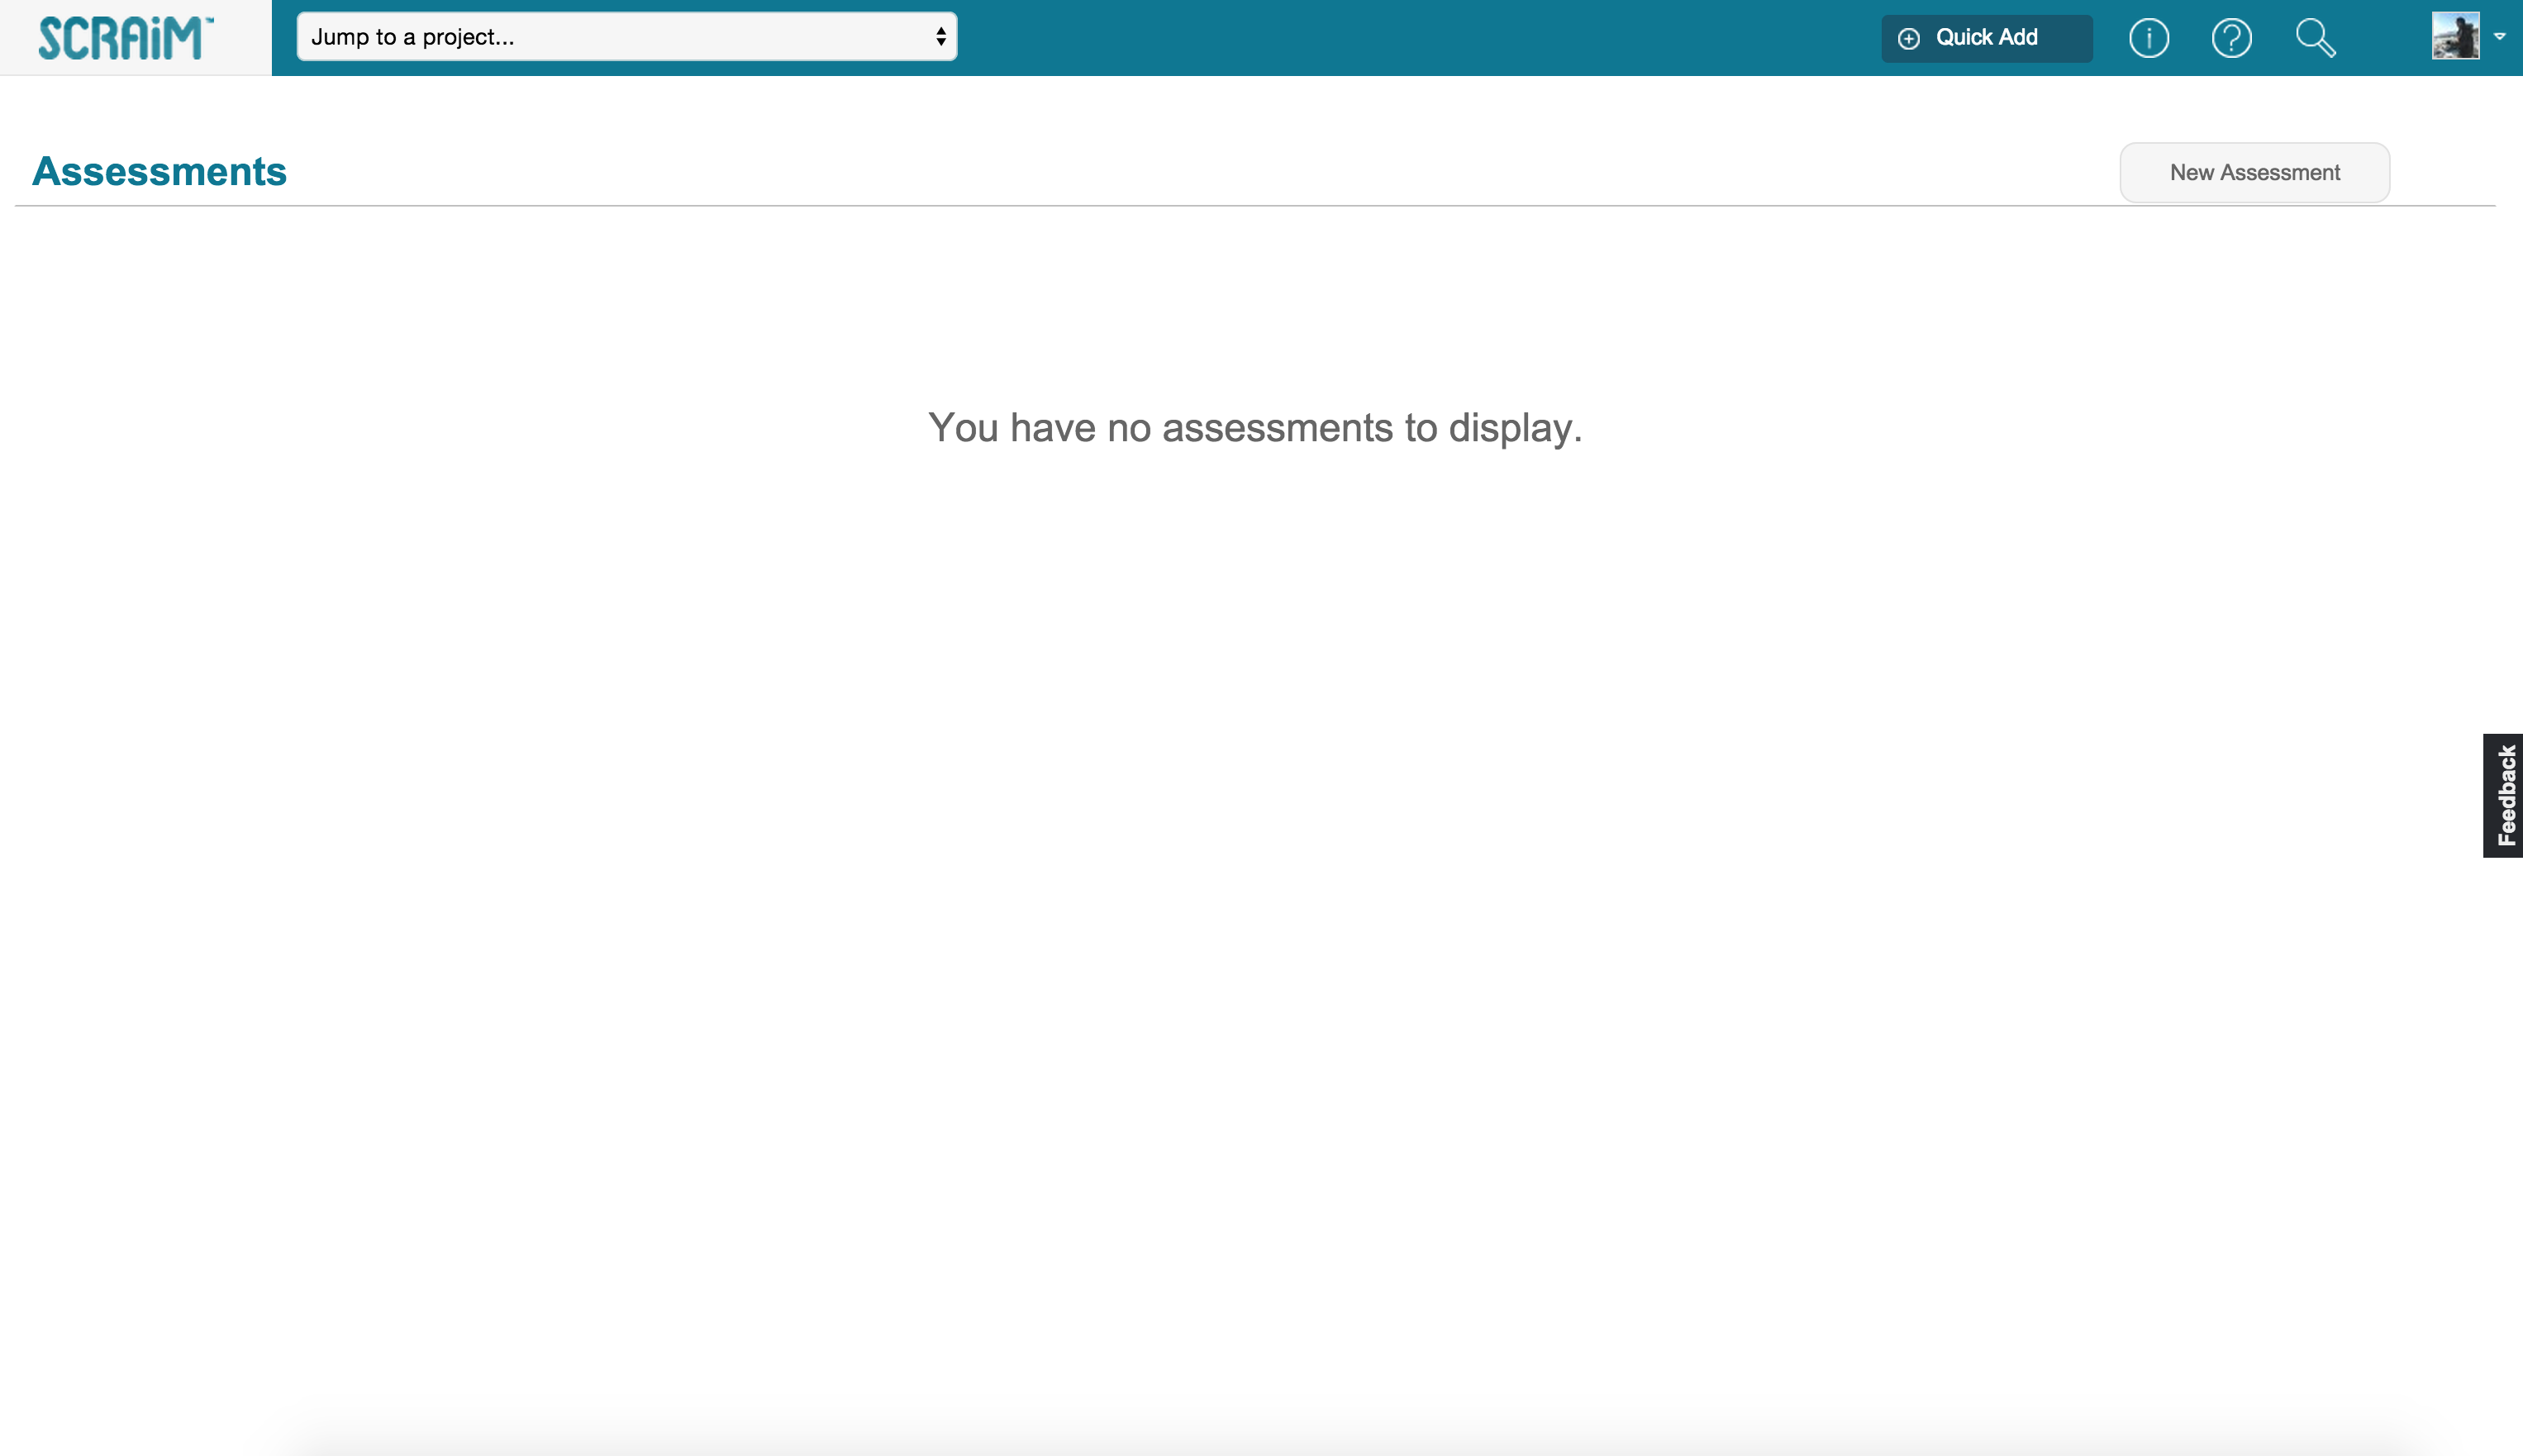
\includegraphics[width=0.9\textwidth]{no_assessments}
		\caption{Homepage without assessments done}
		\label{fig:no_assessments}
	\end{center}
\end{figure}

This screen is shown when we don't have assessments performed. If there are some done in this screen is presented a list of the assessments, like in the Figure \ref{fig:done_assessments}. In the Image, the three assessments are shown by ascending date order, so on bot are the most recent assessments.

\begin{figure}[!htb]
	\begin{center}
		\leavevmode
		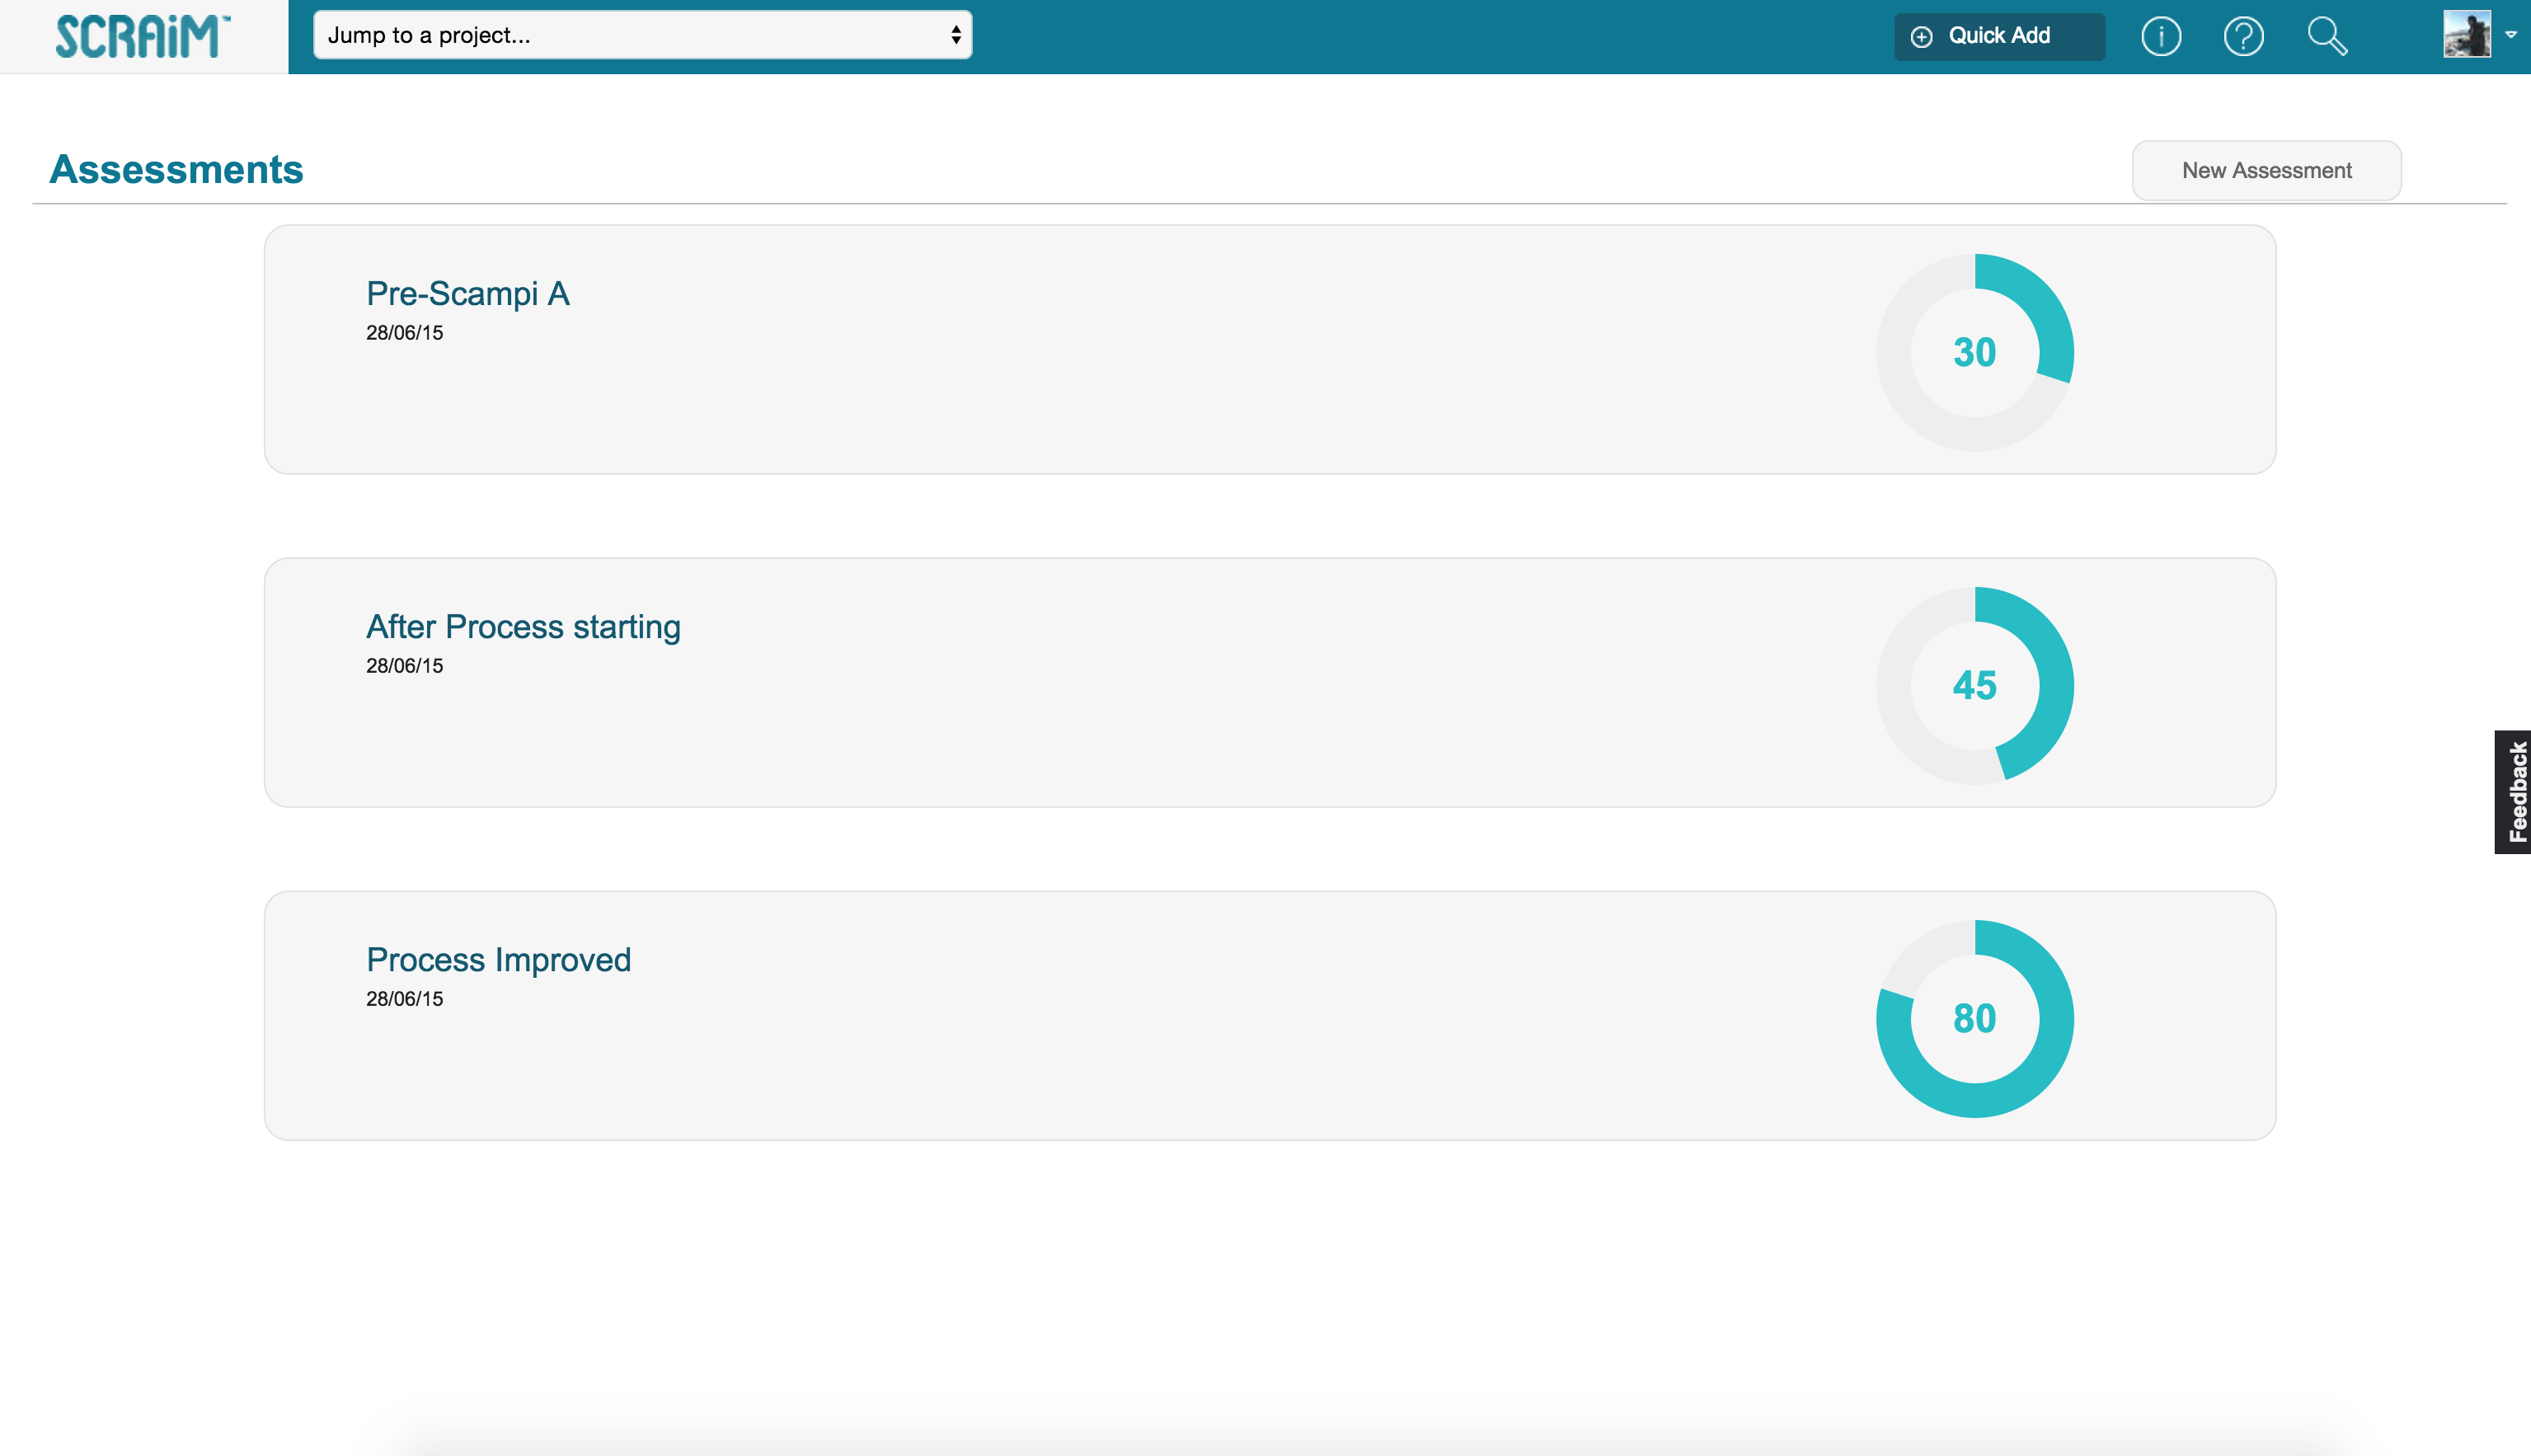
\includegraphics[width=0.9\textwidth]{done_assessments}
		\caption{Homepage with three assessments done}
		\label{fig:done_assessments}
	\end{center}
\end{figure}


\vspace{10 mm}

\textbf{Assessment Options}

In the Figure \ref{fig:done_assessments}, on the right top corner there is a button that says "New assessment". When that button is pressed the application leads us to a screen where is prepared the assessment. This preparation screen can be seen in the Figure \ref{fig:prepare_assessment}, in this page is needed to specify the name of the assessment if we want a custom name for the assessment. If the name is not specified a automatic name will be generated with the performed time and date of the assessment. Is needed too choose the project or projects that are going to be evaluated.

\begin{figure}[!htb]
	\begin{center}
		\leavevmode
		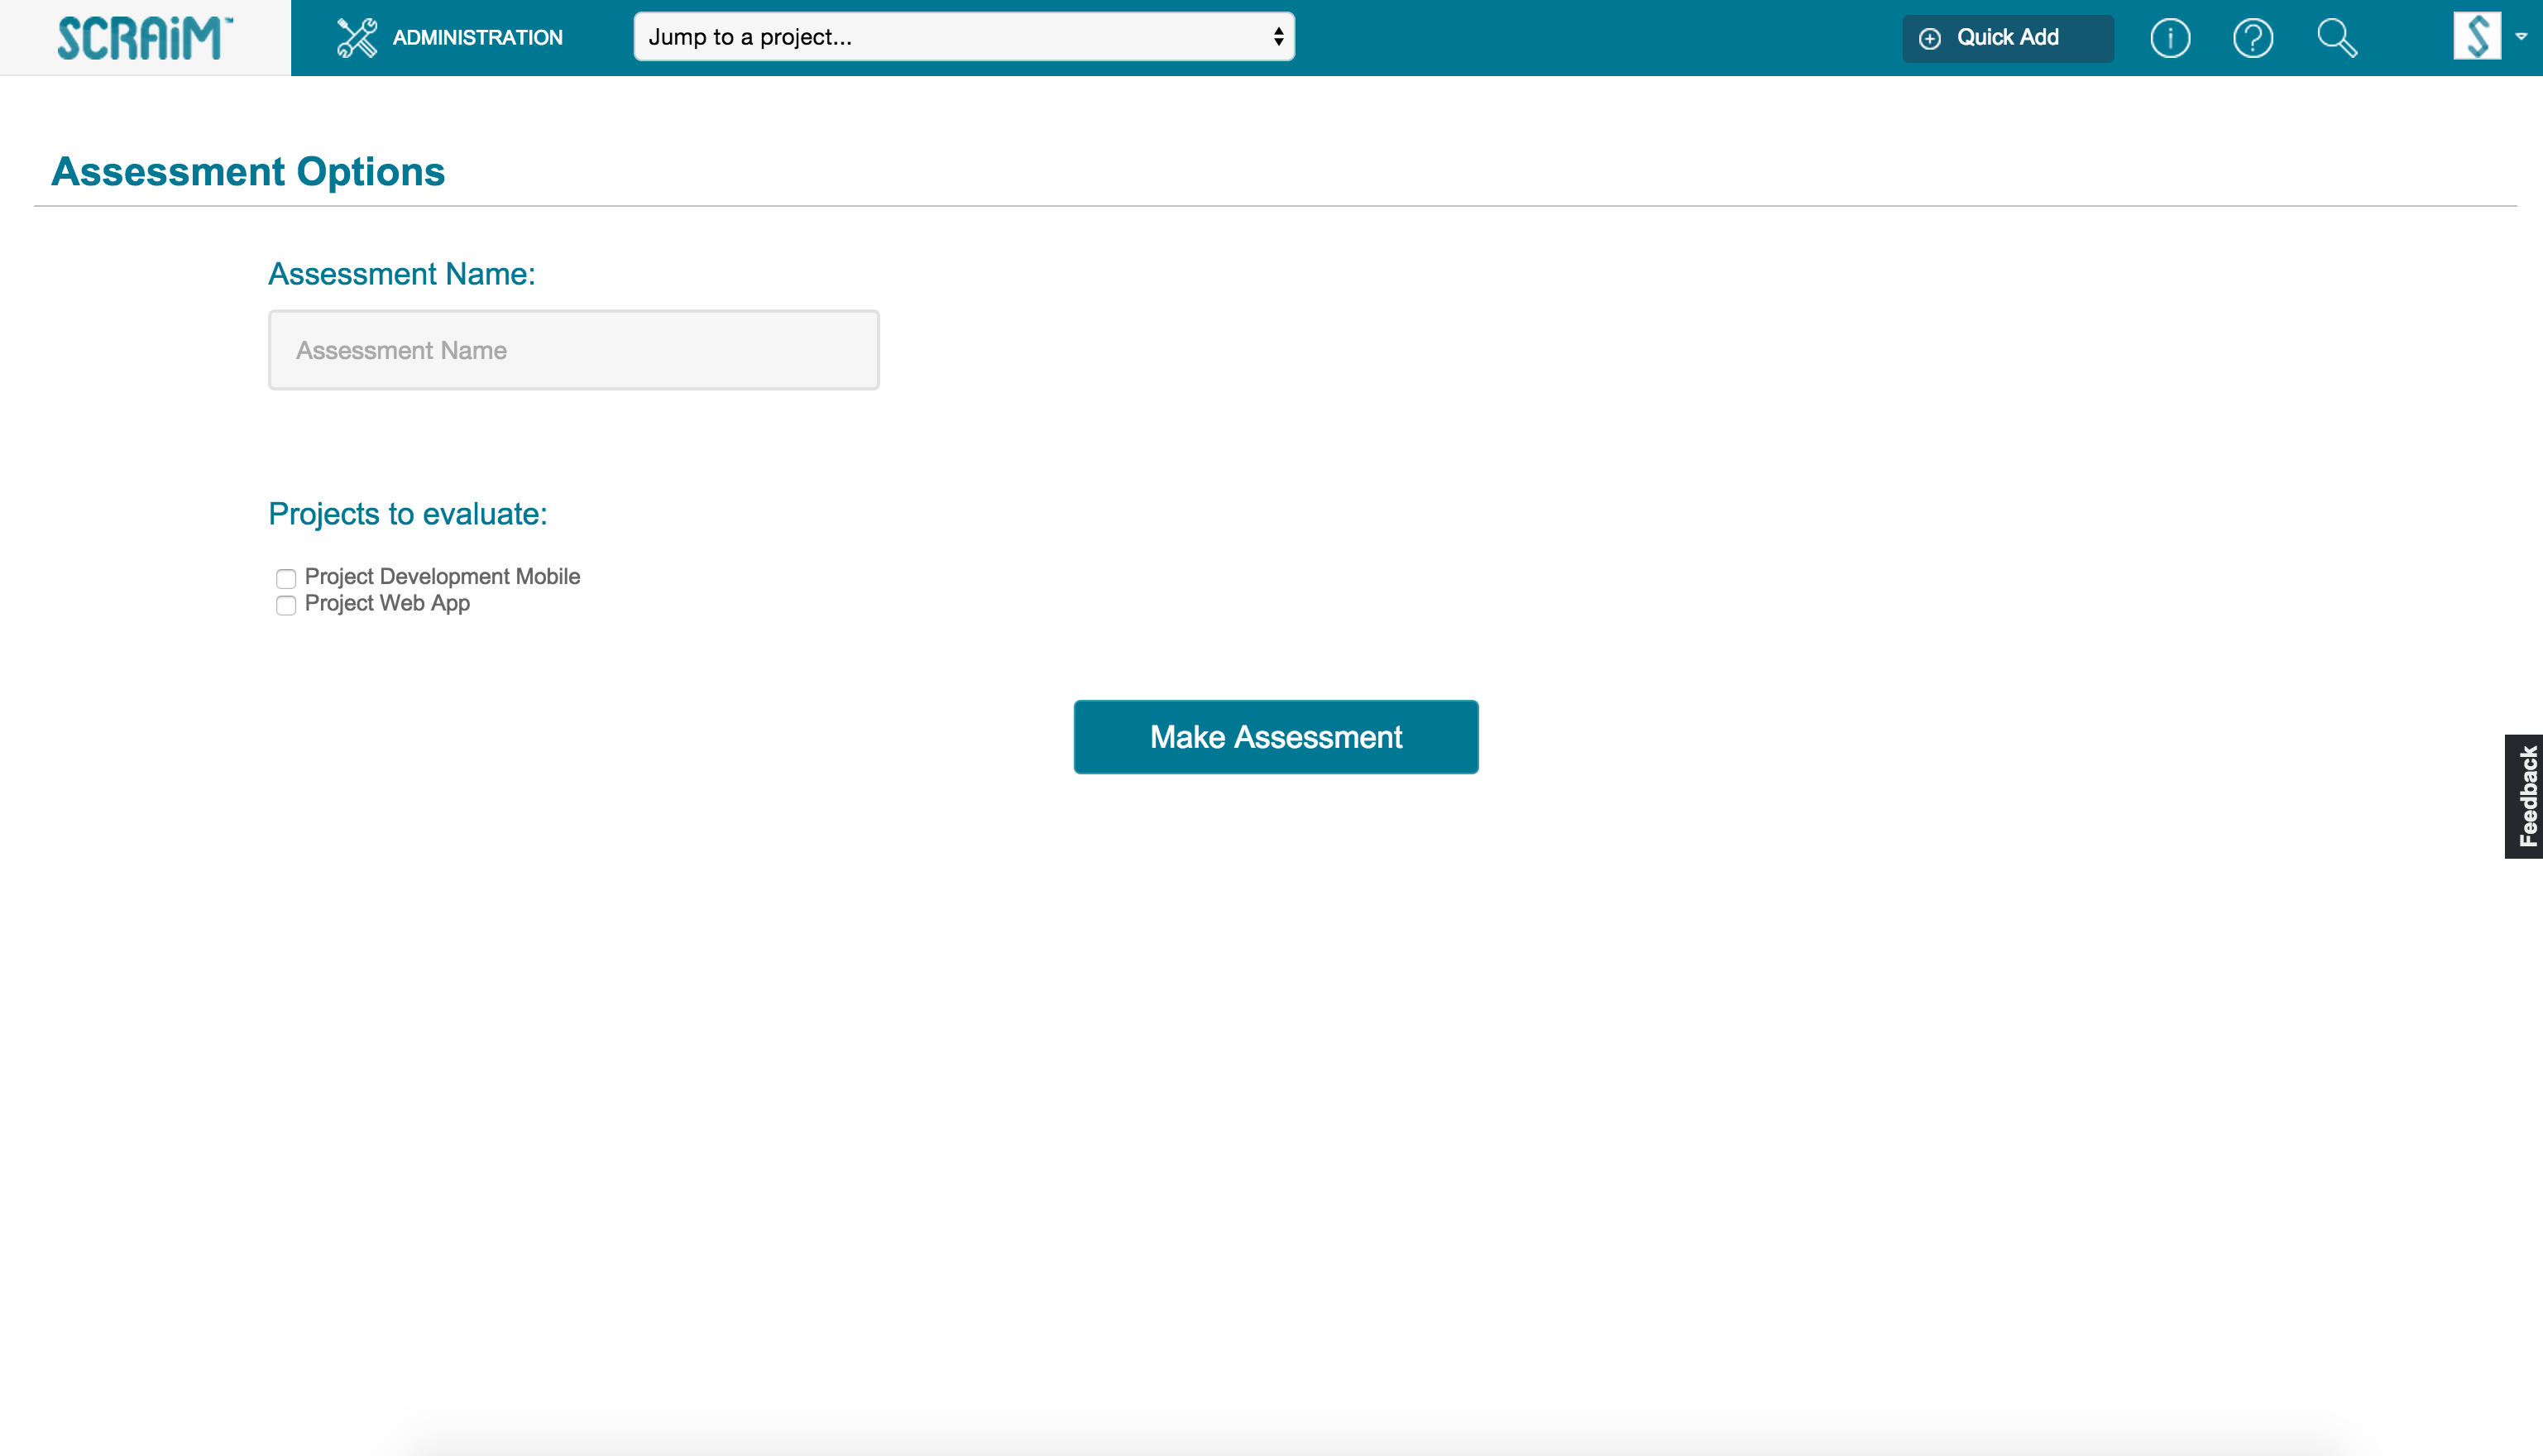
\includegraphics[width=0.9\textwidth]{prepare_assessment}
		\caption{Homepage without assessments done}
		\label{fig:prepare_assessment}
	\end{center}
\end{figure}

Only the text field can be empty, is mandatory to choose at least one project. After completing this process, the button make assessment can be clicked and that will lead us to the screen presented in the Figure \ref{fig:goto_survey}.

\vspace{10 mm}

\textbf{Survey Screen}

\begin{figure}[!htb]
	\begin{center}
		\leavevmode
		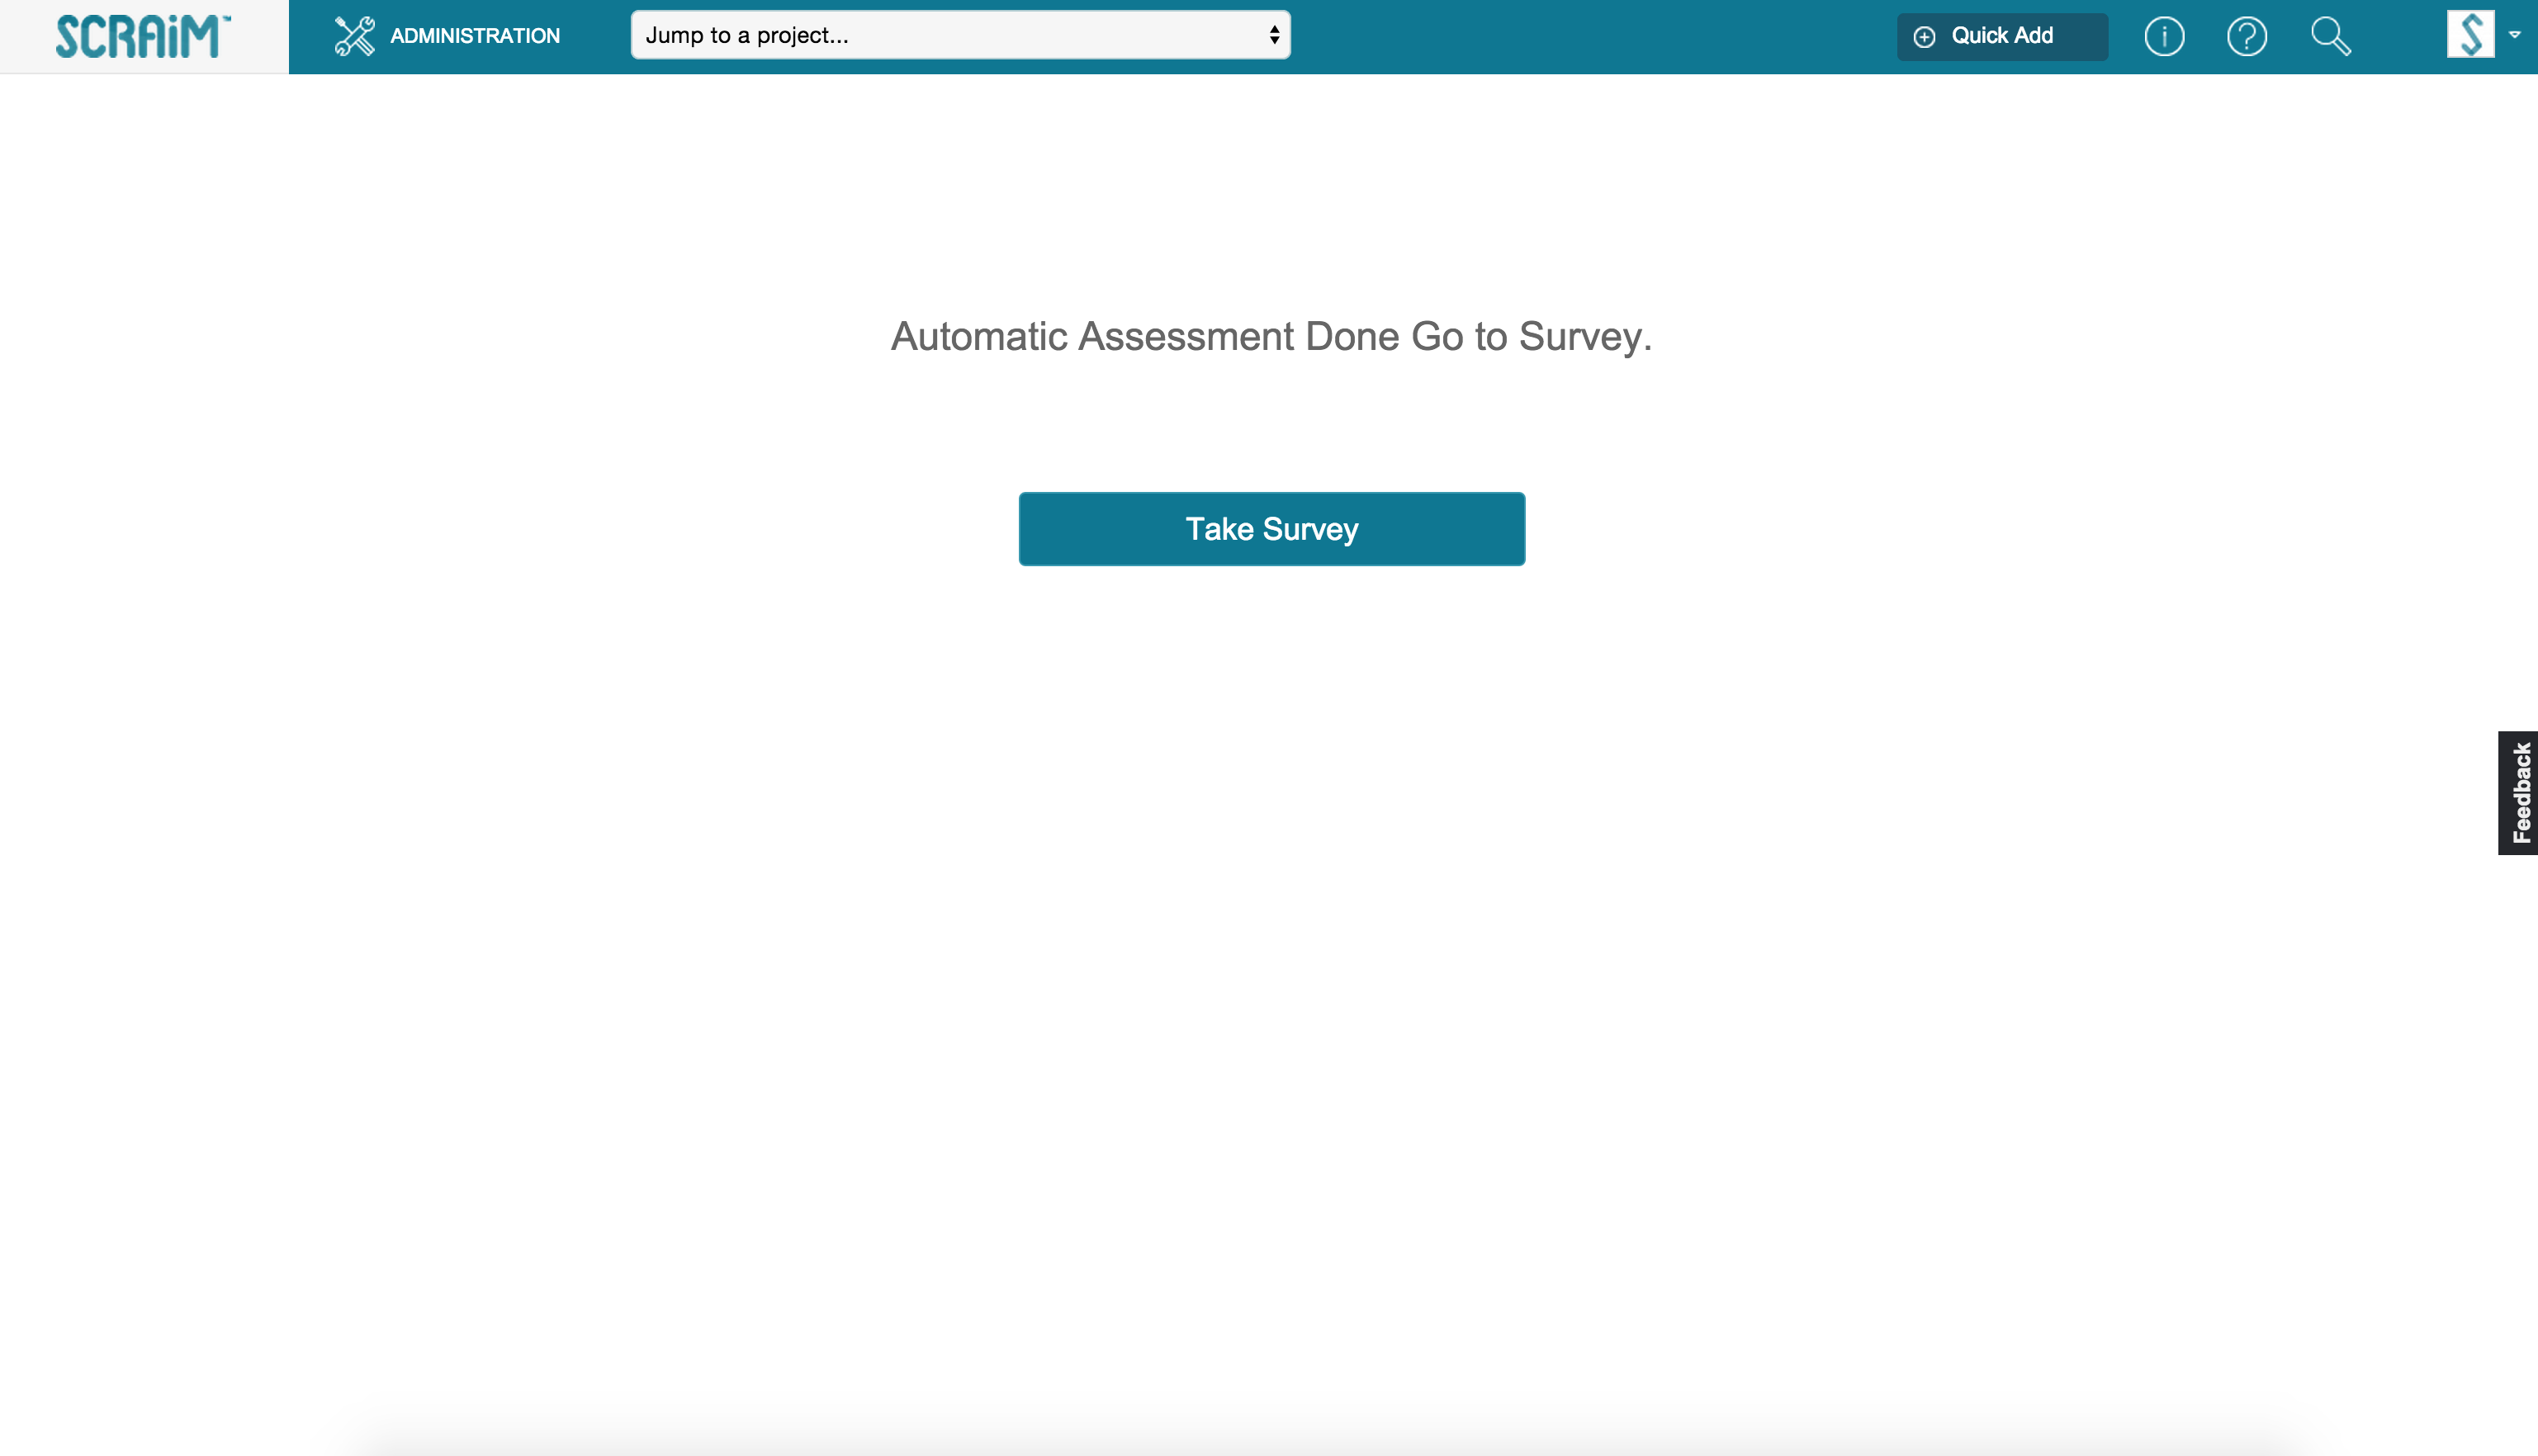
\includegraphics[width=0.9\textwidth]{goto_survey}
		\caption{After Automatic Assessment, needed Survey}
		\label{fig:goto_survey}
	\end{center}
\end{figure}

The Survey is the Screen where is needed to answer all the questions, none can be skipped and only after that we can have a full assessment done and a proper result.

\vspace{10 mm}

\textbf{Results}

When all the process is completed we can see the results obtained, the results can be viewed in the Figure \ref{fig:area_view}. In this screen we can see the result of a project per area, in this case is only contemplated the areas Process Monitoring and Control and Project Planning.

\begin{figure}[h]
	\begin{center}
		\leavevmode
		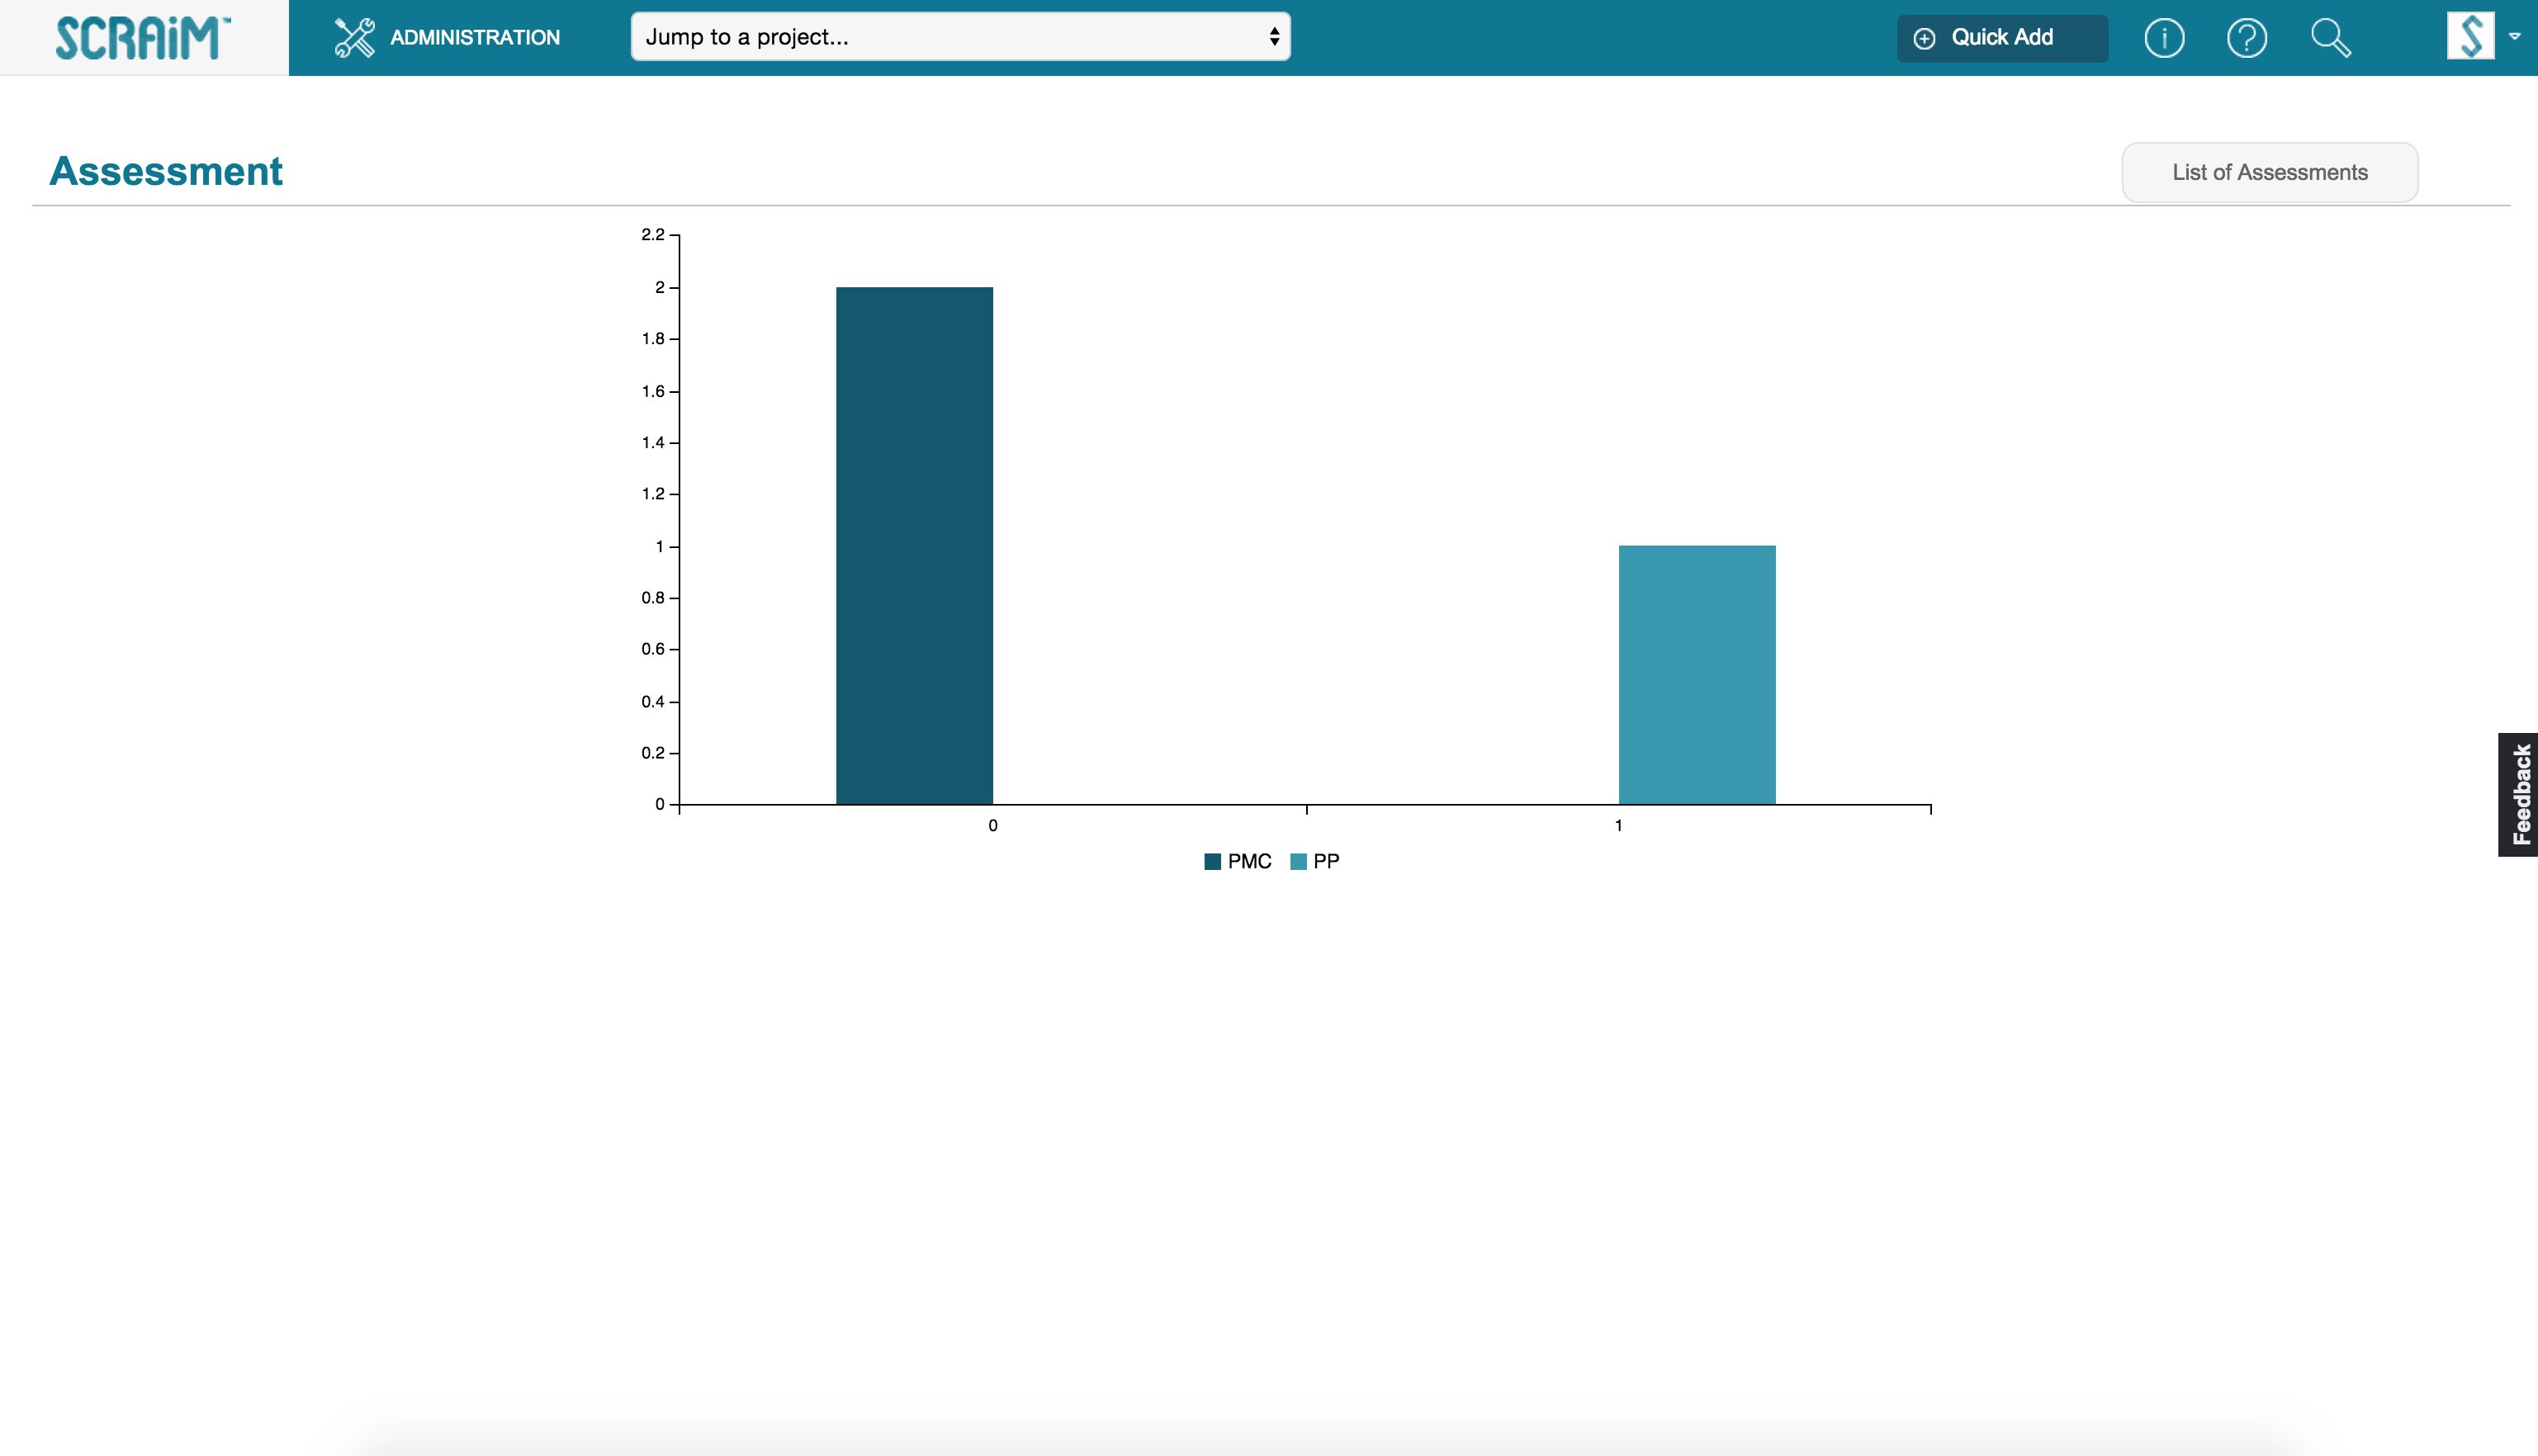
\includegraphics[width=0.9\textwidth]{area_view}
		\caption{Result of assessment, area view}
		\label{fig:area_view}
	\end{center}
\end{figure}

When inside the graph a certain area is clicked, like for example PP which stands for Project Planning, the content of the graph changes to the practices results, that can be checked in the Figure \ref{fig:practices_view}.


\begin{figure}[!htb]
	\begin{center}
		\leavevmode
		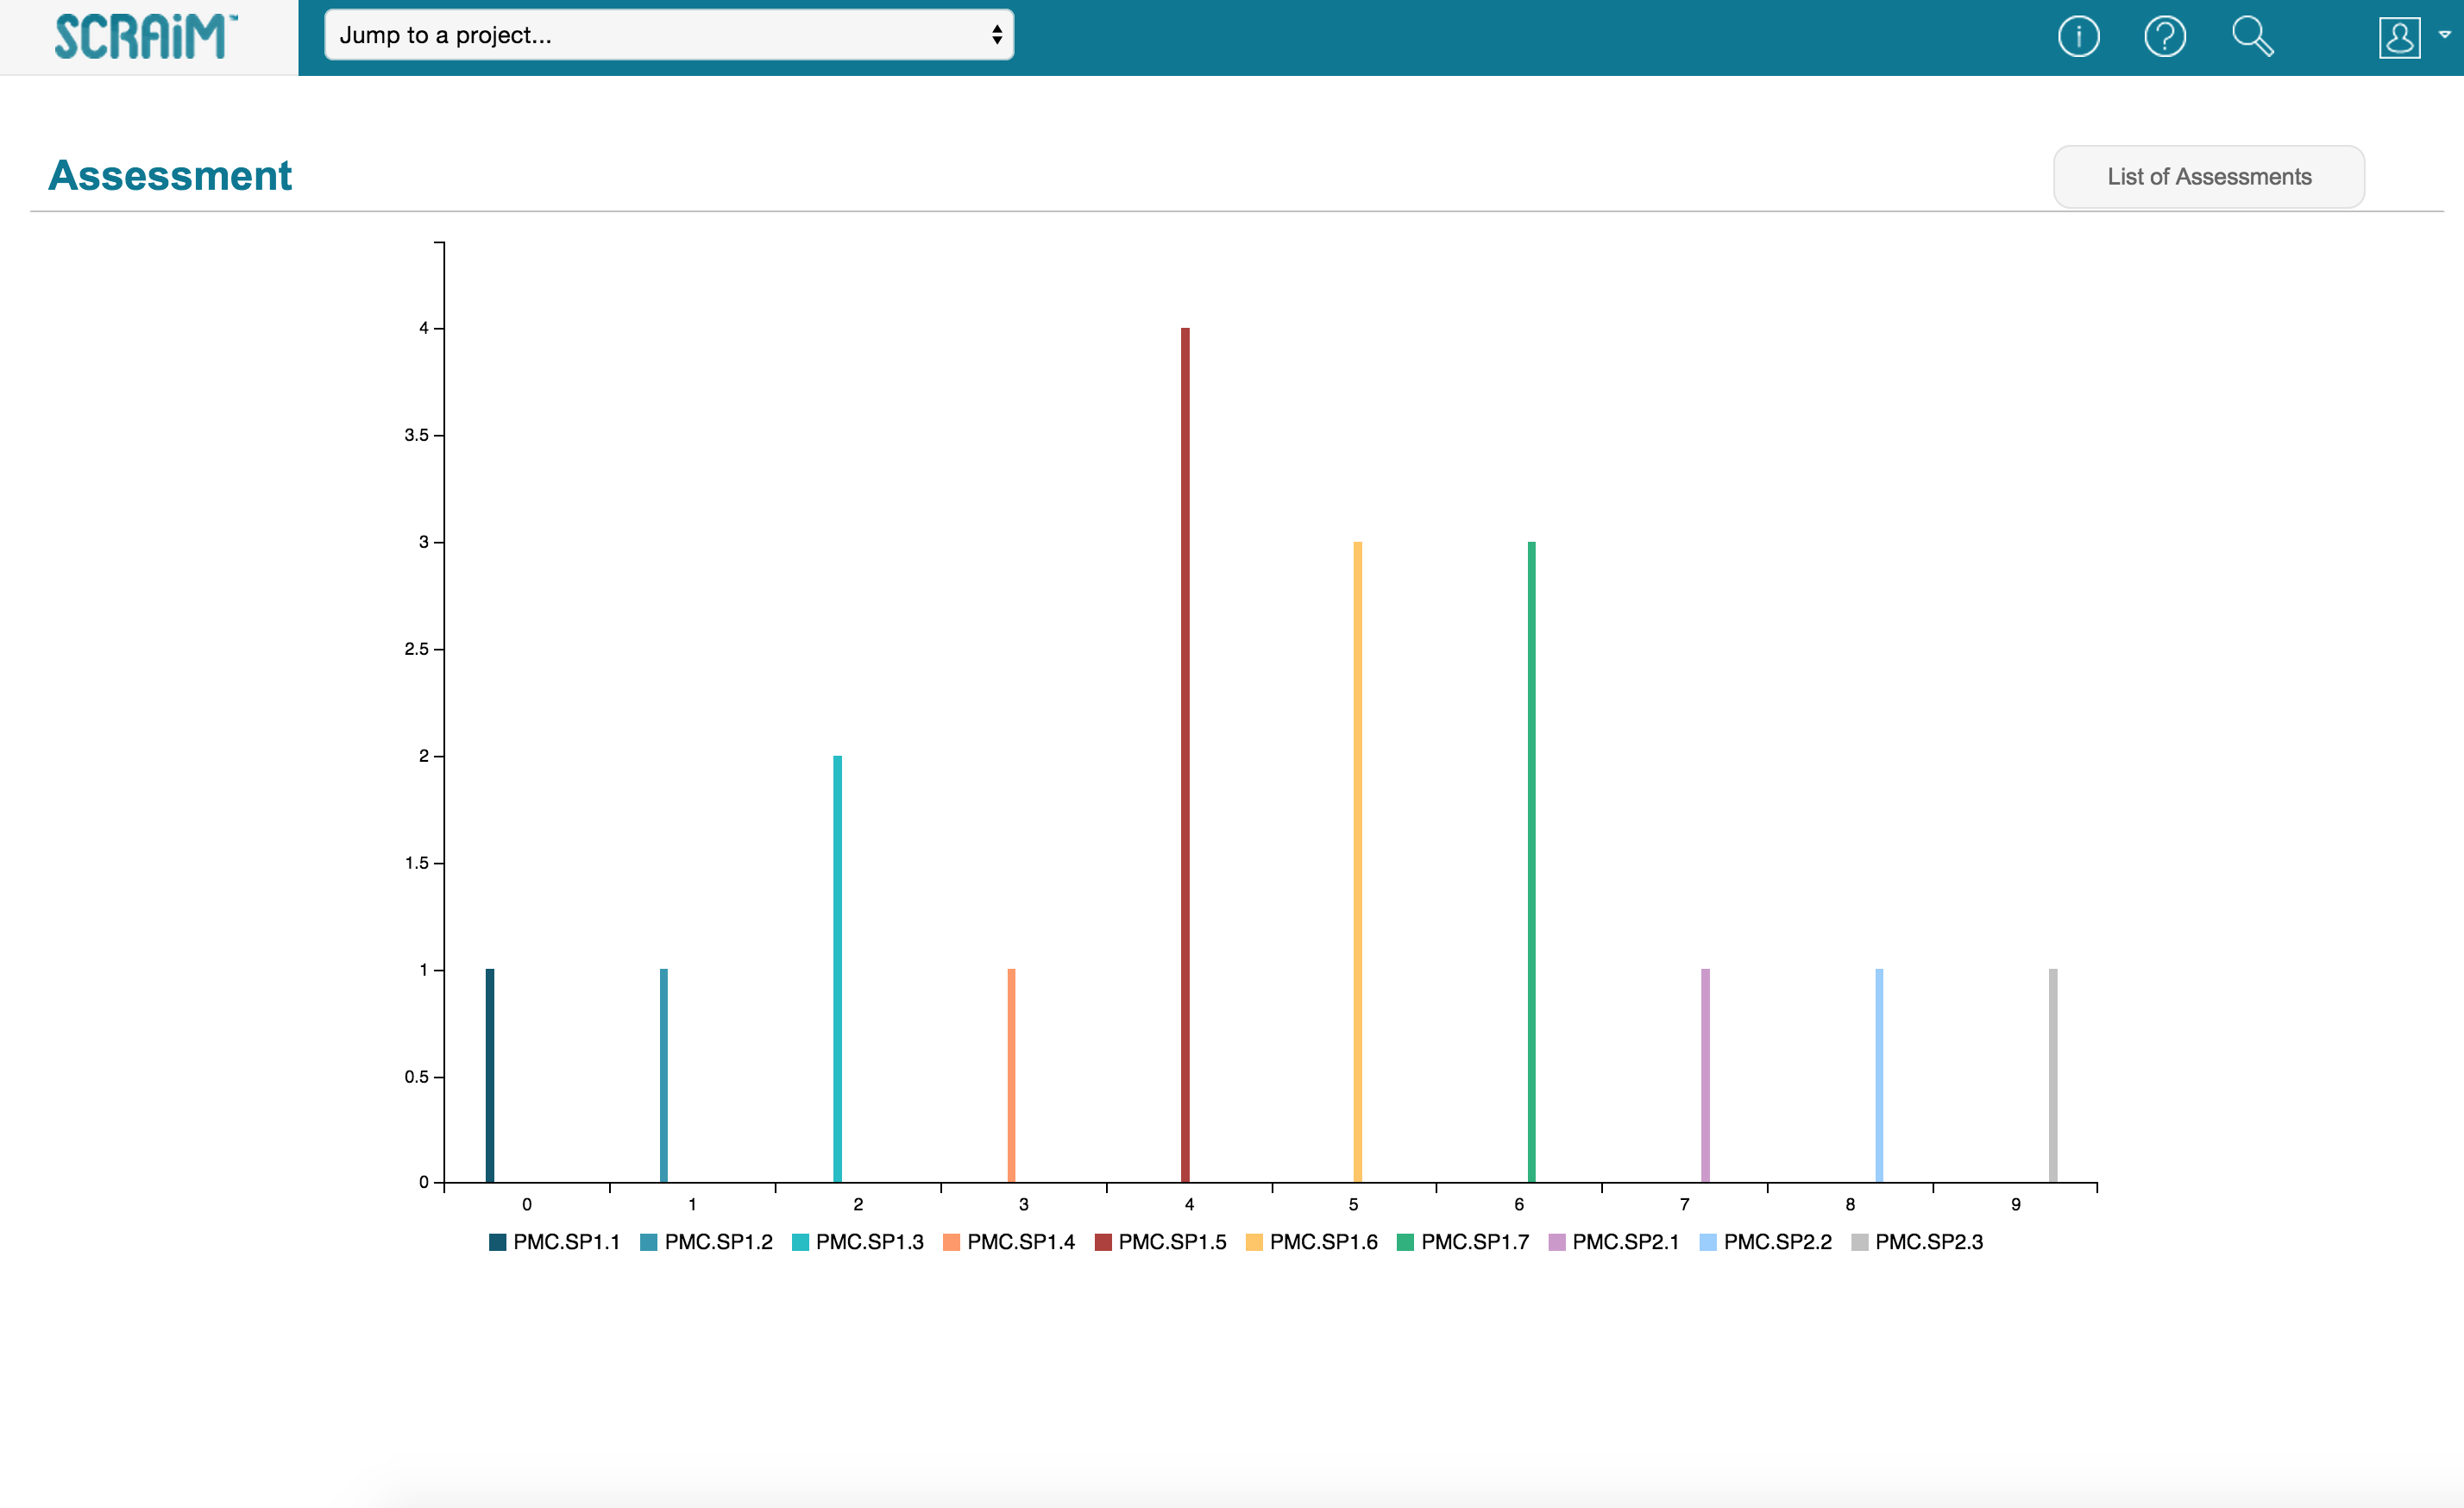
\includegraphics[width=0.9\textwidth]{practices_view}
		\caption{Result of assessment, practices view}
		\label{fig:practices_view}
	\end{center}
\end{figure}

Is possible to see more in detail the assessment result if the mouse cursor is over the bar that correspond to a practice, when that bar is clicked, is shown in the page more info about that practice. The Figure \ref{fig:practice_click}, shows us the information appended to the page when the Practice 1.1 of the first goal of Project Planning Area is clicked.

\begin{figure}[!htb]
	\begin{center}
		\leavevmode
		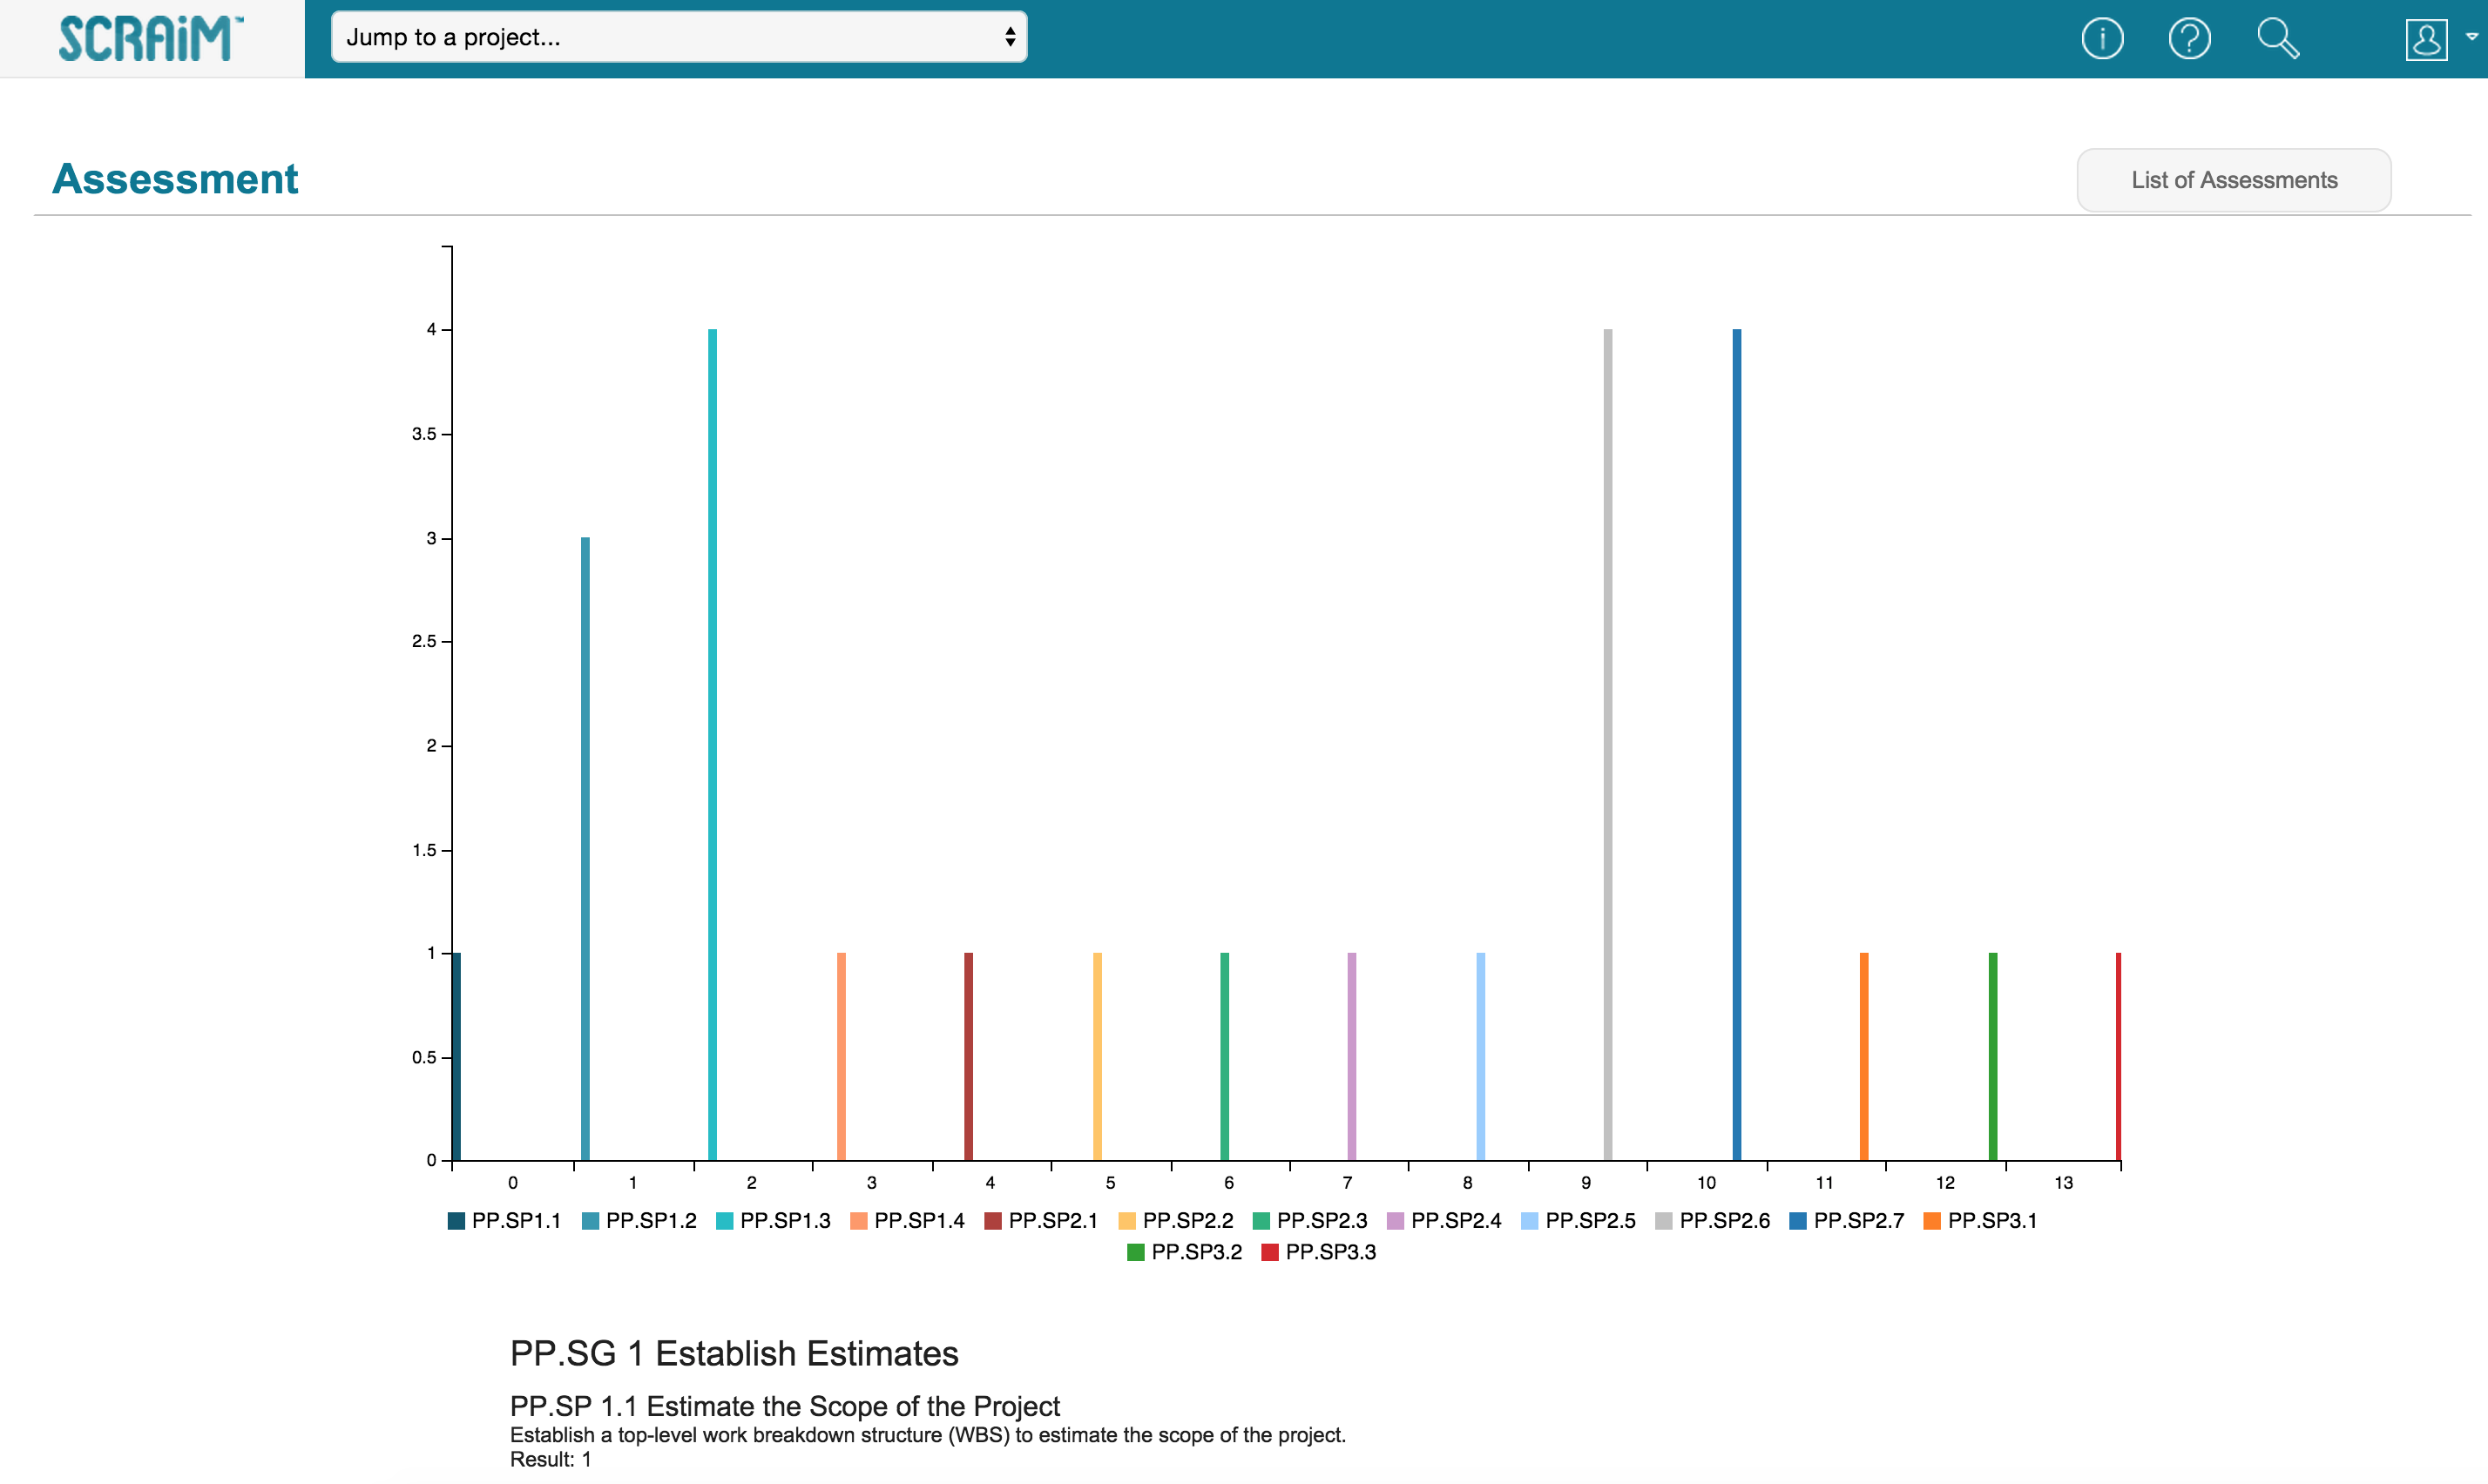
\includegraphics[width=0.9\textwidth]{practice_click}
		\caption{Result of assessment, practice view details}
		\label{fig:practice_click}
	\end{center}
\end{figure}

After all this process, all views are able to return to the Home screen, that contains the list of the assessments done, the assessment that we have done and we are seeing is already present on the list of assessments.

\section{Coverage percentage} \label{sec:coverage}

%Scraim extension to increase cmmi coverage

%Implementação até onde está neste momento falar das duas àreas totalmente implmentadas - PP e PMC

Despite the conception and the mapping of all Areas from second maturity level of CMMI for development, this prototype of the set of tools and methodologies only contemplates the implementation of two areas on the tool.

The Implemented areas are Project Planning and Project Monitoring and Control, those areas are the areas that is possible to get more feedback from the automatic part of the assessment. 
 
\section{Comparison between Automatic and Manual assessment} \label{sec:automatic}
%	Avaliação manual vs automatica trocar titulo

To determine if the implemented module is close to a real assessment is necessary to compare an automatic assessment (tool) to a manual assessment (human).

For that purpose is chosen a project that is already finished and instantiated on SCRAIM.
In both assessments we can see that only the two areas featured on the implementation of this module are object of this comparison.

\begin{figure}[!htb]
	\begin{center}
		\leavevmode
		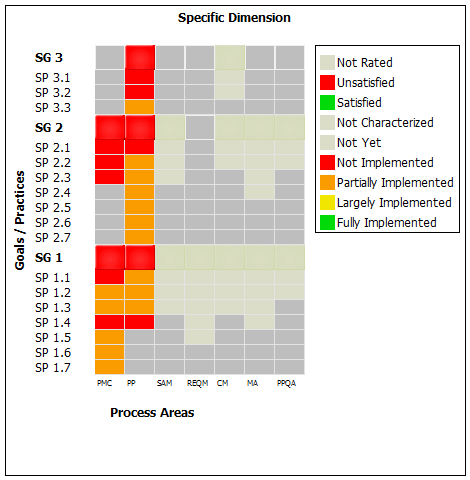
\includegraphics[width=0.9\textwidth]{manual_assessment}
		\caption{Manual assessment, done for one appraisal}
		\label{fig:manual_assessment}
	\end{center}
\end{figure}

\textbf{Manual Assessment}

The Manual assessment that is shown in Figure \ref{fig:manual_assessment} was performed by a Consultant from Strongstep.

In the manual assessment we can see that in Project Planing for the first goal only the last practice is not implemented and the others practices are Partially implemented. For the second goal all practices are partially implemented except the first one.
In the third goal only the last practice is partially implemented the others are not implemented.

For the area Project Monitoring and Control in the first goal the first and forth practices are classified as not implemented and the other as partially implemented. In the second goal all practices are not implemented.

\textbf{Automatic Assessment}

The Automatic assessment performed by the developed module can be seen in Figure \ref{fig:automatic_assessment}.

\begin{figure}[!htb]
	\begin{center}
		\leavevmode
		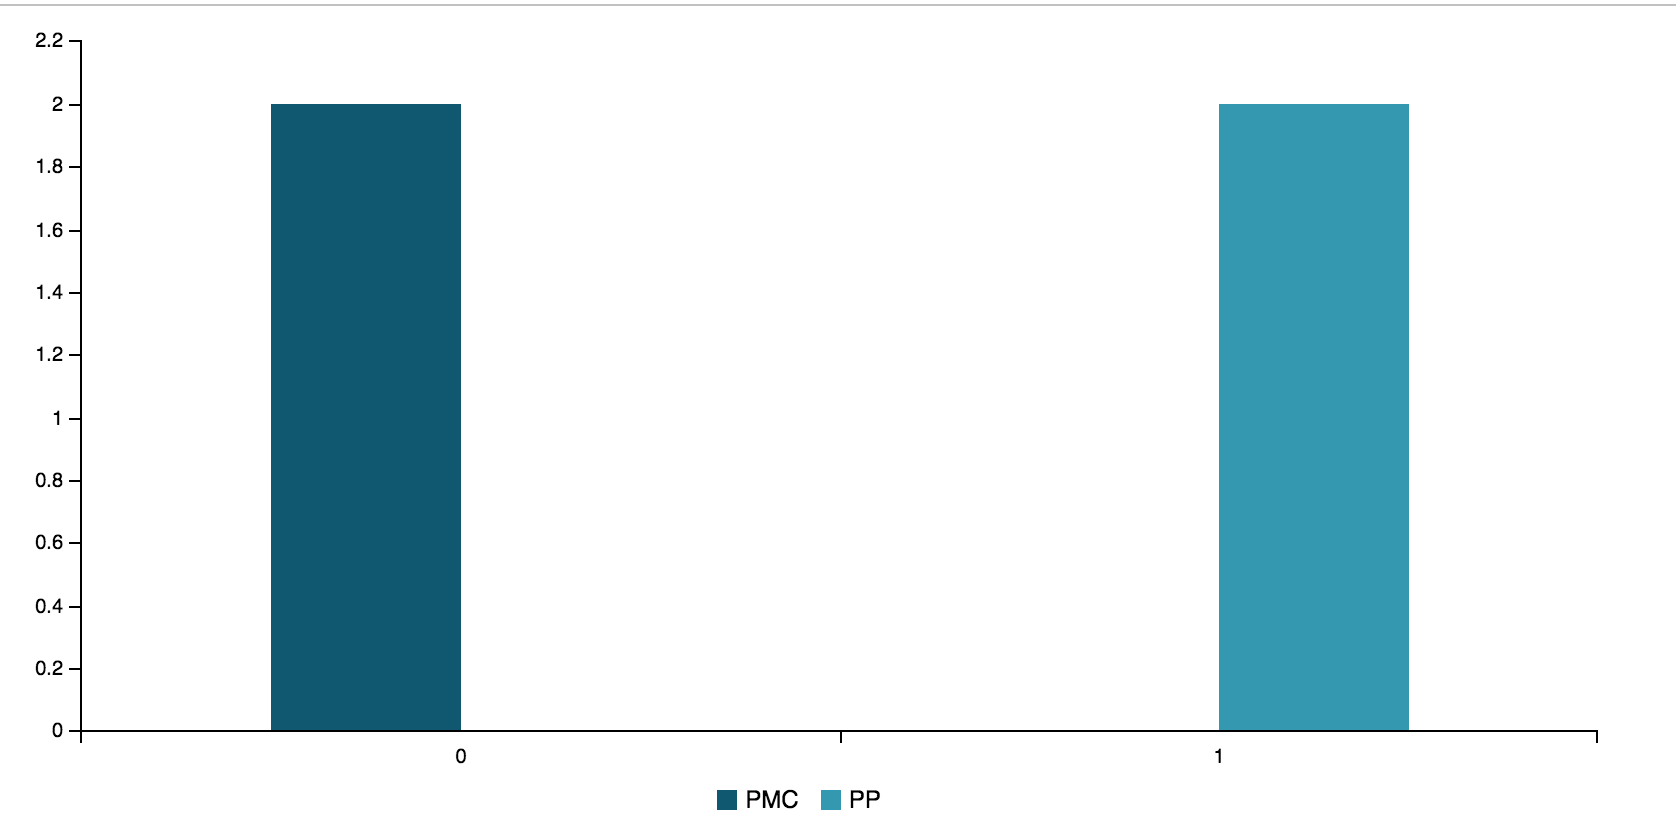
\includegraphics[width=0.9\textwidth]{automatic_assessment}
		\caption{Scraim Automatic Assessment}
		\label{fig:automatic_assessment}
	\end{center}
\end{figure}

In Figure \ref{fig:automatic_assessment} is presented the assessment of the two areas, in this case the assessment result for the areas of PP and PMC are 2 and 2 in the SCRAIM scale.

For the PP area, the practices results are shown in Figure \ref{fig:results_pp}.

Using for method of approximation the scale presented in Section \ref{sec:mapping} and comparing the automatic results with the Manual assessment shown before is possible to say in the most cases the mapping of the tool matched the manual assessment. In some cases like  the SP.2.2 the risks of the project weren't recorded on SCRAIM but in a document attached to the project.


Results for PMC area are represented in Figure \ref{fig:results_pmc}. Using the same method that used before and comparing the two results, none practice stands out from the results, so the results are close to a real assessment.


\begin{figure}[!htb]
	\begin{center}
		\leavevmode
		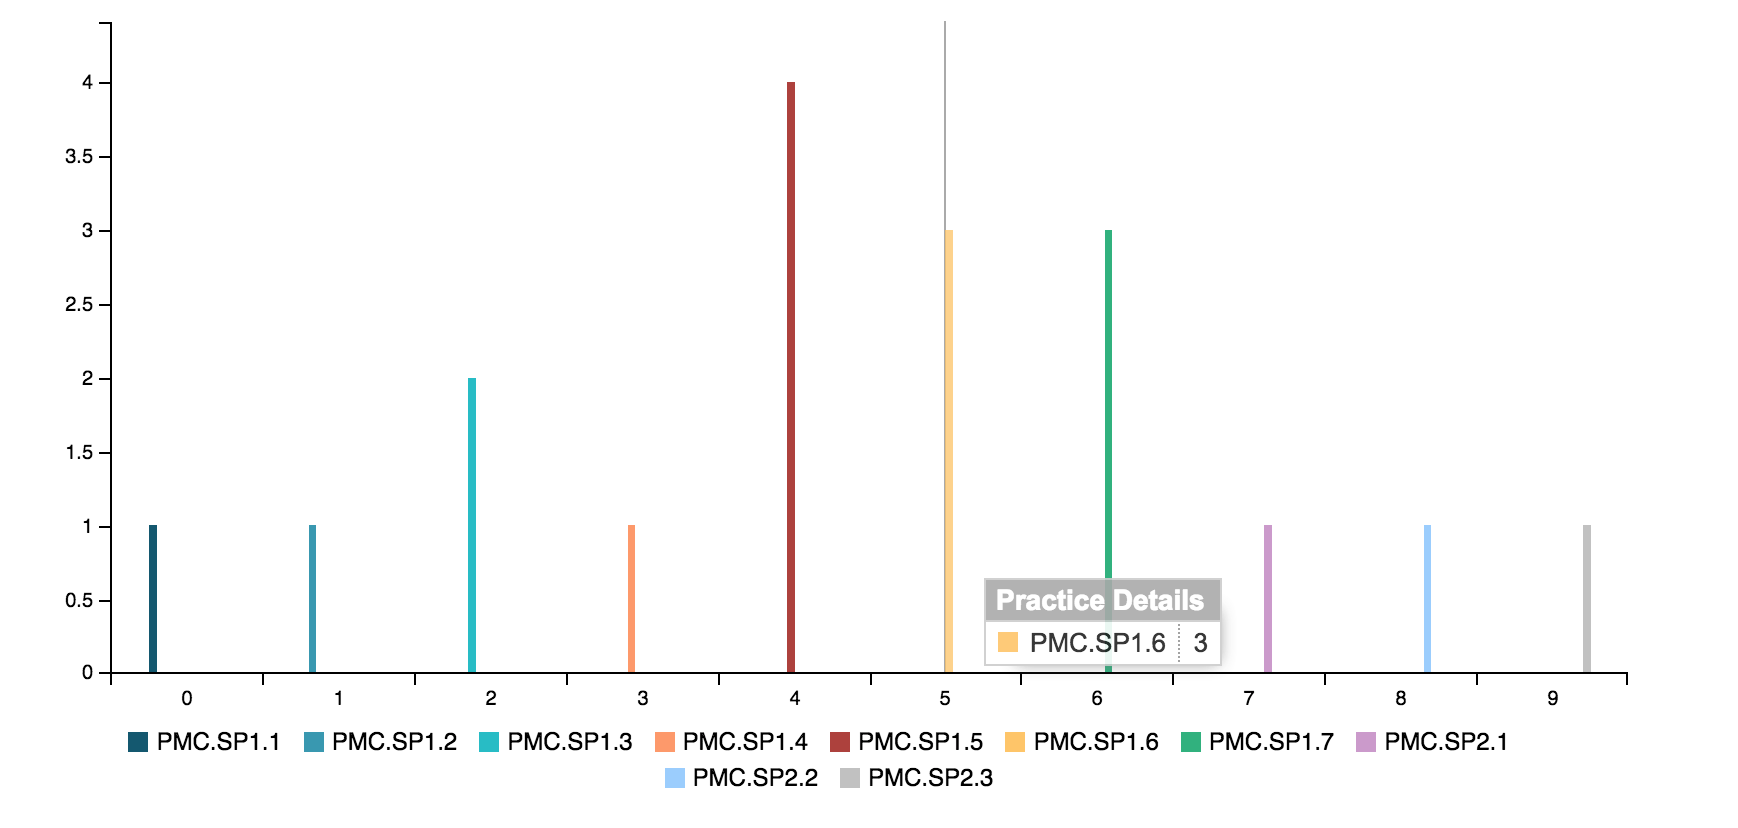
\includegraphics[width=0.9\textwidth]{results_pmc}
		\caption{Project Monitoring Control Results}
		\label{fig:results_pp}
	\end{center}
\end{figure}

\begin{figure}[!htb]
	\begin{center}
		\leavevmode
		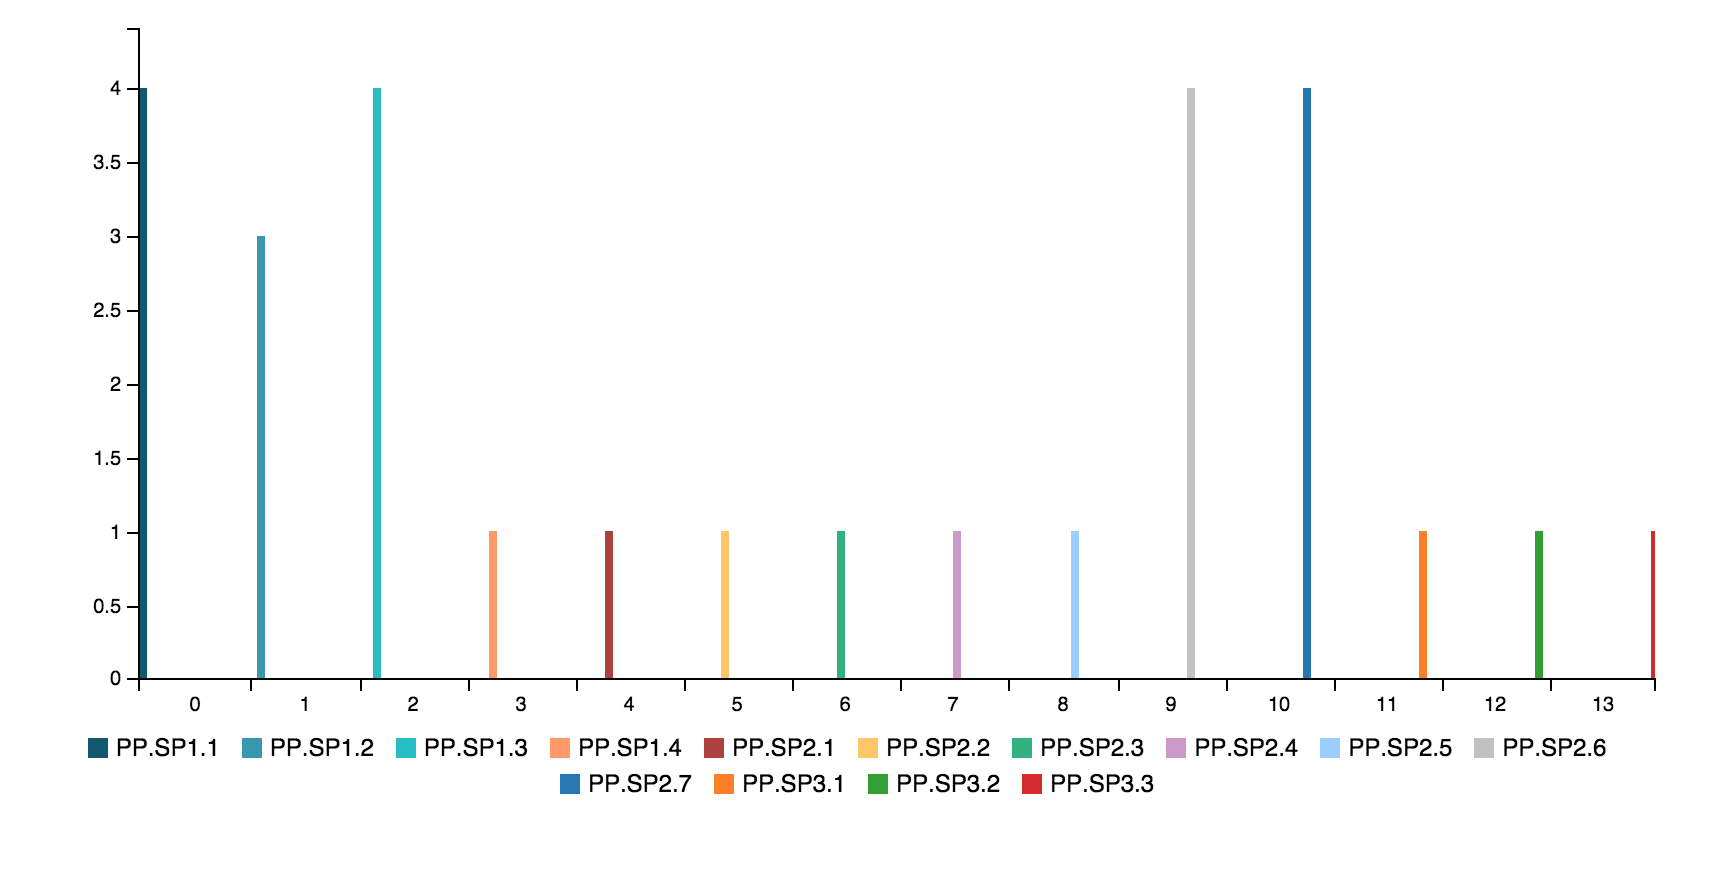
\includegraphics[width=0.9\textwidth]{results_pp}
		\caption{Project Planning Results}
		\label{fig:results_pmc}
	\end{center}
\end{figure}